\chapter{Modeling an Image Collection - Setup}
\label{sec:experimental_setup}

This chapter describes an application of the models presented in the Chapter \ref{sec:models} to a real dataset. As mentioned in the introduction, finding and recommending paths for tourists is an interesting research topic. These paths can be understood as spatial summaries of a city, representing the most important locations to visit and photograph in a city.

These tourist paths can be discovered from a large collection of geotagged images by using the accompanying timestamps as explained in section \ref{sec:path_discovery}. Even though these paths are naturally ordered, they can also be used as unordered sets of locations that represent the behavior of different visitors taking photographs in the city, which can be modeled using the FLID, FLDC and FFLDC models. The modeling quality of these proposed models was compared to other existing methods from the literature as explained in section \ref{sec:baselines}. The procedure used for evaluating the results are described in section \ref{sec:evaluation}.

\section{Flickr Dataset}

For the experiments on real data, public geotagged photos from Flickr were used. There are close to two million geo-tagged photos available on Flickr\footnote{https://www.flickr.com/map reports 1,833,307 geotagged photos as of April 9th, 2016.}, this offers an unique and rich dataset for the problem of spatial summarization. But as described before, this work focuses on the city level. Therefore, the experiments were performed on a subset of the Flickr data, namely on public geotagged photos taken within Zürich, Switzerland.

The Flickr API\footnote{\url{https://www.flickr.com/services/api/}} provides multiple functions to explore and use the data, in particular the search endpoint allows developers to retrieve photo records according to a specific criteria. Each photo record contains the following information:

\begin{description}
  \item[Owner] The ID of the user who uploaded and owns the photo.
  \item[Title] A title given by the user.
  \item[Description] A description given by the user.
  \item[Visibility] Indicates if a photo is public, private or semi-private, i.e. shared only with friends.
  \item[Dates] Dates when the photo was taken, uploaded and last modified.
  \item[Geo] Indicates if the photo is geotagged, the geotag's precision, latitude and longitude.
  \item[License] Copyright license.
  \item[Tags] Text tags set by users.
  \item[Machine tags] Automatic text tags set by Flickr.
  \item[URL] The URL to download the photo. 
\end{description}

Most of these properties can be used to filter the search results, for collecting the desired data for Zürich the following criteria was used:

\begin{itemize}
  \item The photo was taken between 2005 and 2015.
  \item The photo is marked as public and has no copyright restrictions.
  \item The photo is geotagged and has street level accuracy. The location of the photo must be within the area shown in Figure \ref{fig:zurich_bb}.
\end{itemize}

\begin{figure}
  \centering
  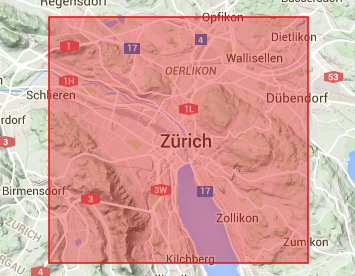
\includegraphics[width=\textwidth]{zurich_bb}
  \caption{Bounding box used for filtering photos taken in the Zürich area.}
  \label{fig:zurich_bb}
\end{figure}

The API sets some limitations on the search function, namely it does not allow more than 3600 requests per hour and it restricts the search results to the first 4000 records. This means that it was not possible to issue a single search request with the outlined criteria, instead the retrieval was done over the course of several hours though single month queries. This ensured that each query had less than 4000 results, hence retrieving all the available records.

This search yielded 168608 photos taken by 6159 users. Figure \ref{fig:random_photos} shows a random sample of these photos.

\begin{figure}
  \centering
  TODO: COLLAGE
  \caption{A random sample of the photos available in the dataset for Zürich.}
  \label{fig:random_photos}
\end{figure}

Figure \ref{fig:heatmap_zurich} shows the distribution of photos taken in 2015. The majority of them is concentrated at the city center also around locations of interest outside the center like Uetliberg, Oerlikon and the Zoo. This indicates that the dataset contains good information regarding the places to visit and take photographs in Zürich. Figure \ref{fig:heatmap_zurich_zoom} shows zoomed in areas around the city showing that the data is mostly concentrated in touristic places like the historic center, where Fraumünster, Grossmünster and the city hall are.

\begin{figure}
  \centering
  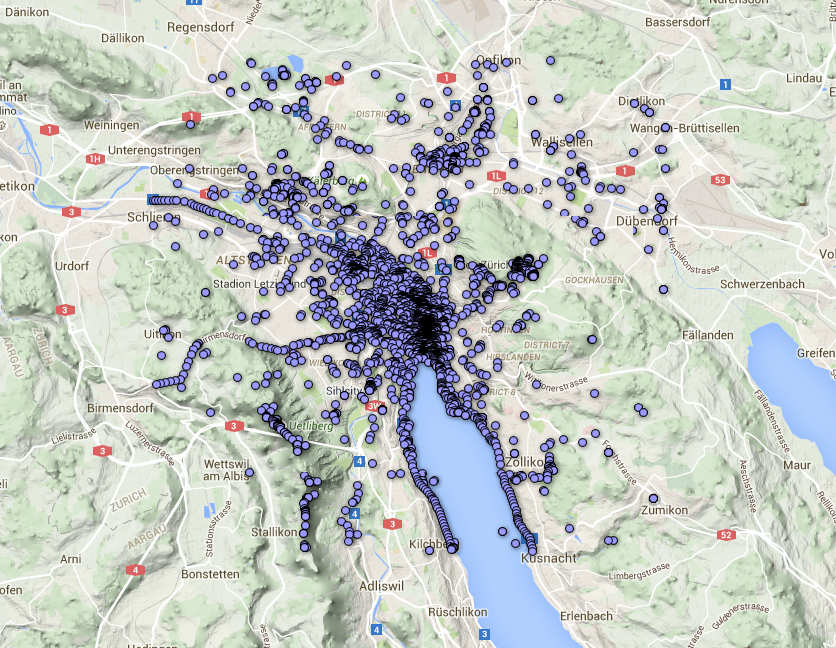
\includegraphics[width=\textwidth]{zurich_feature_map_2015}
  \caption{Feature map with the photos from the Zürich dataset taken in 2015.}
  \label{fig:heatmap_zurich}
\end{figure}

\begin{figure}
  \centering
  \begin{subfigure}[b]{0.45\textwidth}
    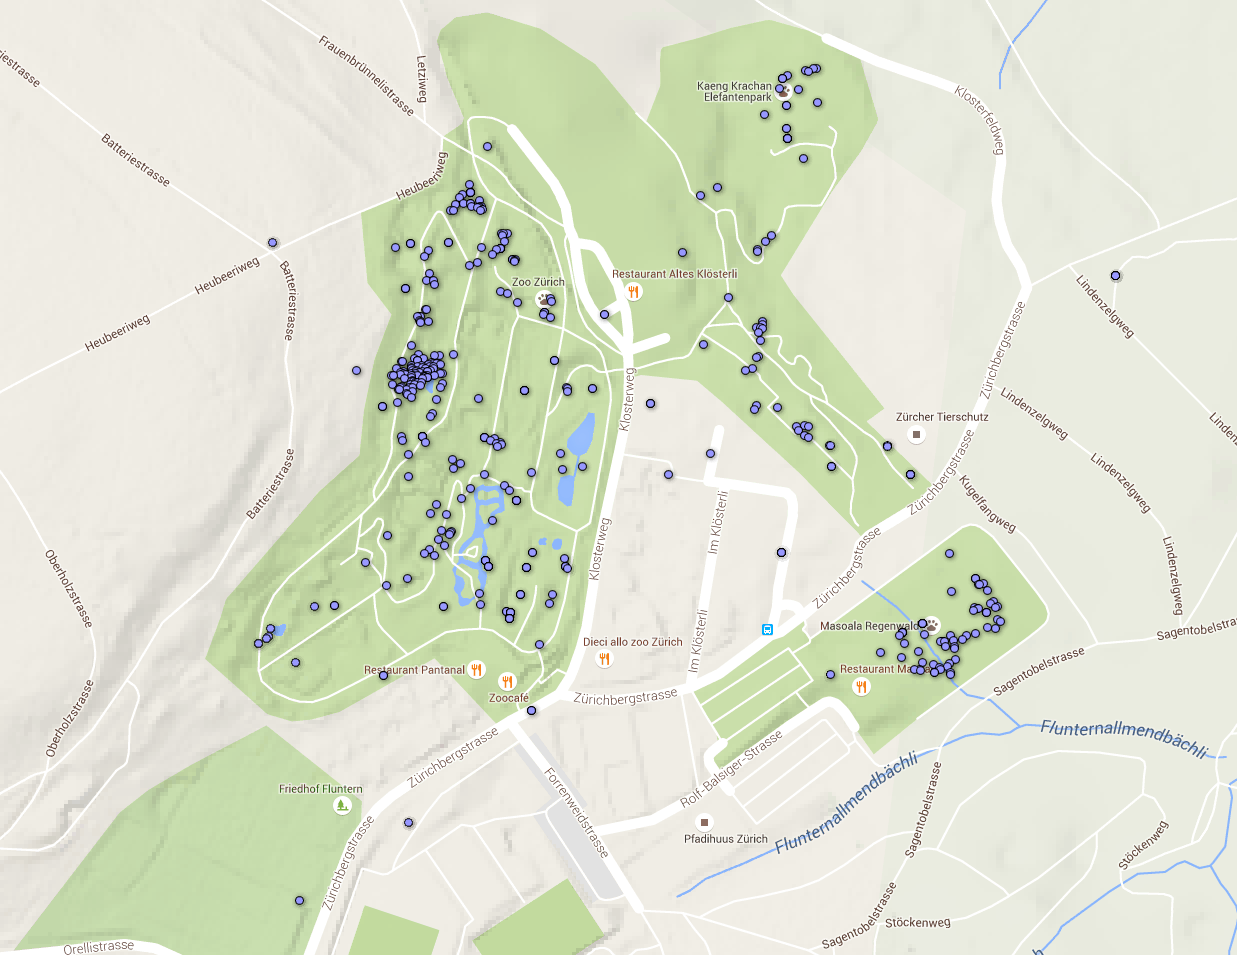
\includegraphics[width=\textwidth]{zurich_zoo}
    \caption{Zürich zoo area.}
  \end{subfigure}
  ~
  \begin{subfigure}[b]{0.45\textwidth}
    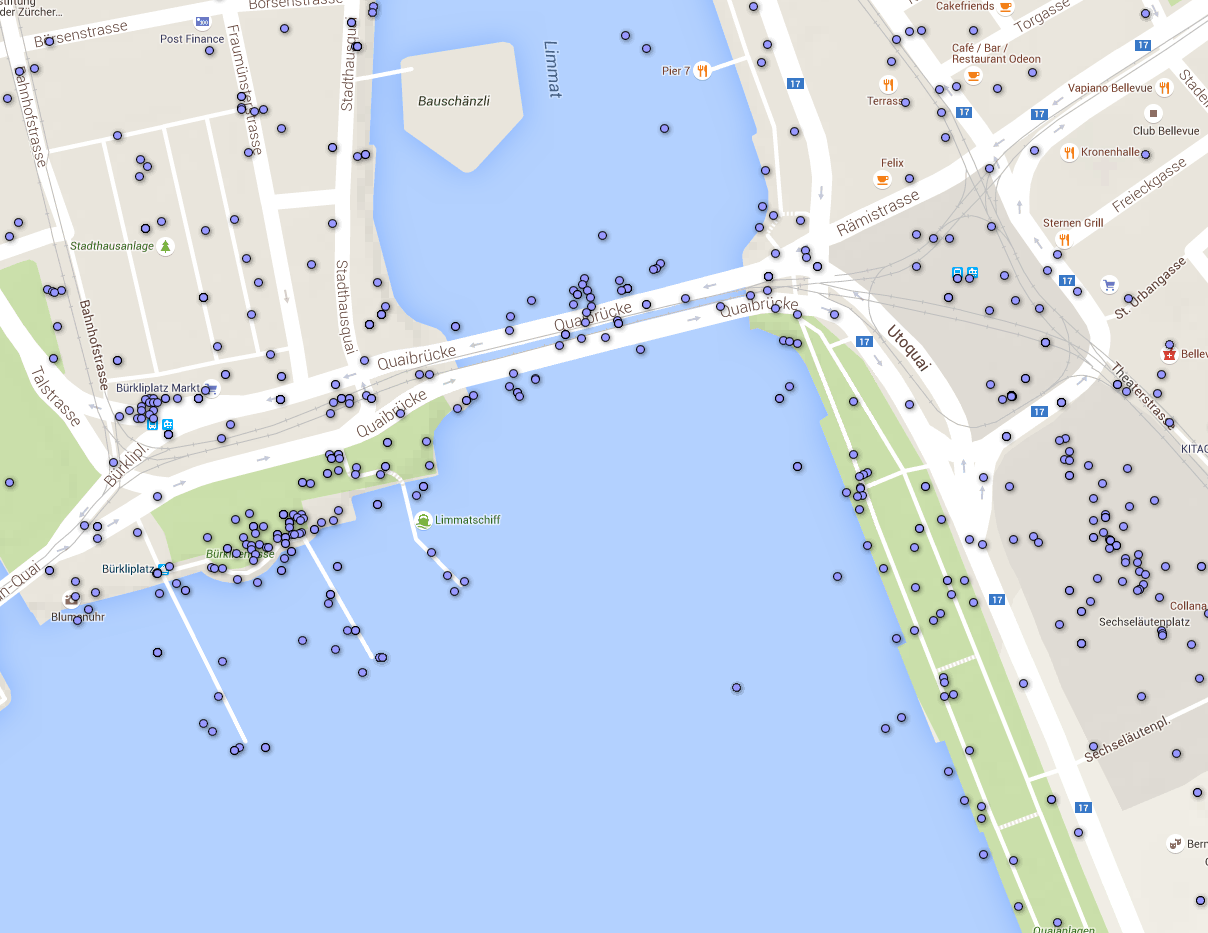
\includegraphics[width=\textwidth]{zurich_burkliplatz}
    \caption{Bürkliplatz area.}
  \end{subfigure}
  \hfill \\
  \begin{subfigure}[b]{0.45\textwidth}
    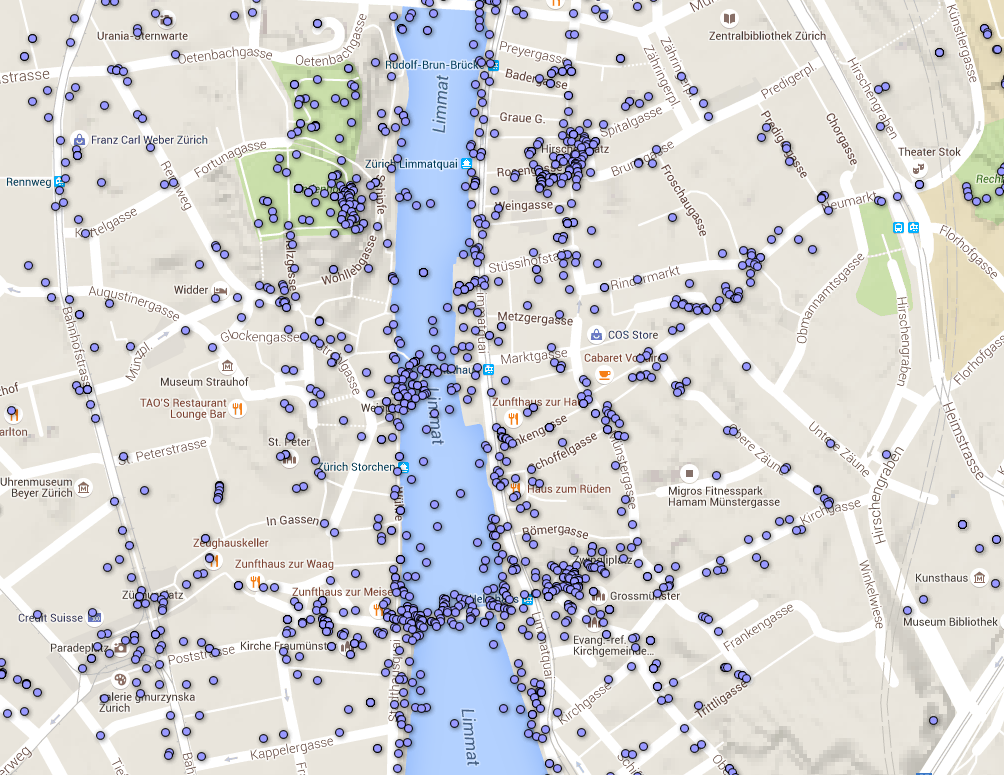
\includegraphics[width=\textwidth]{zurich_center}
    \caption{Historic center area.}
  \end{subfigure}
  ~
  \begin{subfigure}[b]{0.45\textwidth}
    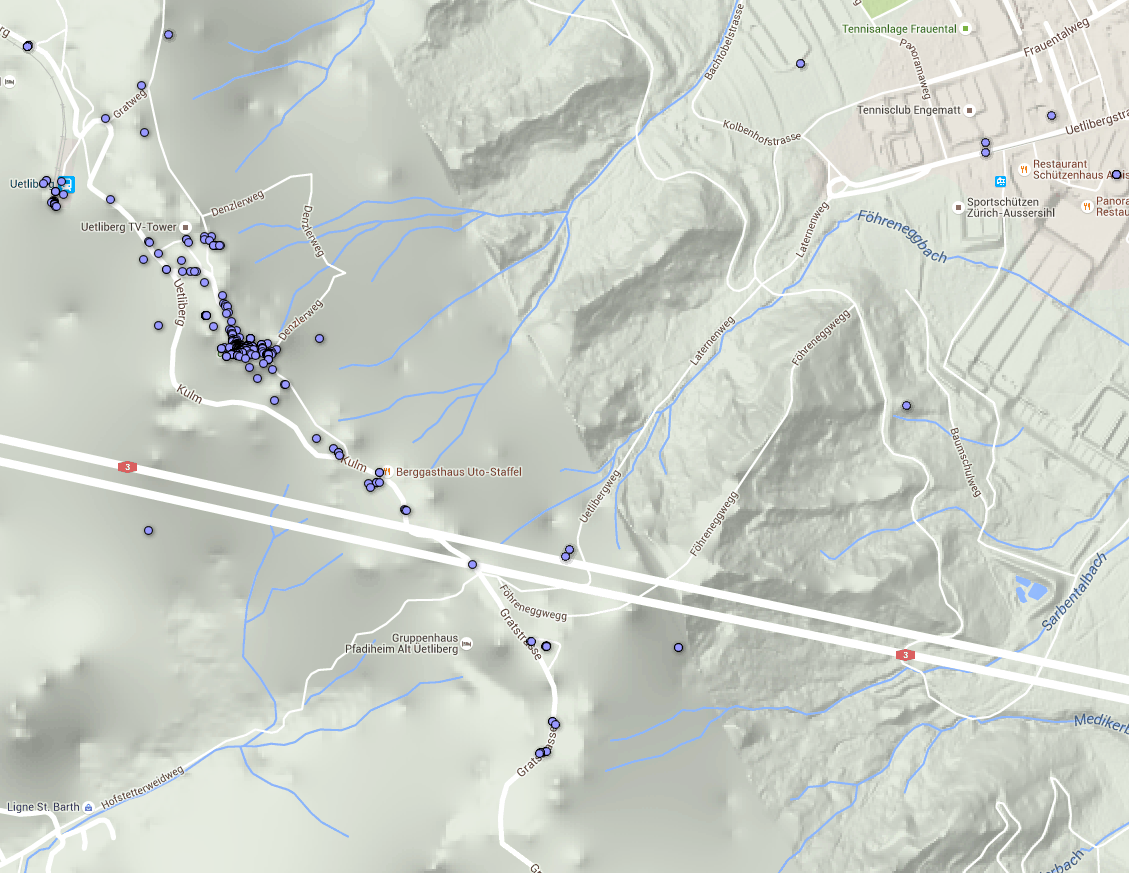
\includegraphics[width=\textwidth]{zurich_uetliberg}
    \caption{Uetliberg area.}
  \end{subfigure}
  \caption{Zoomed in maps displaying popular locations in Zürich.}
  \label{fig:heatmap_zurich_zoom}
\end{figure}

Additional to the spatial coverage of the dataset, one interesting property to explore is how the photos are distributed across users. The histogram of photos taken by each user is shown in figure \ref{fig:photo_user_distribution}, this is cut off at 100 photos because the distribution has a heavy tail that is unimportant. This heavy tail is due to professional users like newspapers and event venues that have uploaded hundreds of photos under a single user, these users are not of particular interest for the use case of this work because they do not reflect the interests of a typical visitor. The histogram shows that most of the users uploaded one or two pictures which indicates that most of the photos come from very active users that take hundred of photos, this should be taken into account when analyzing the results.

\begin{figure}
  \centering
  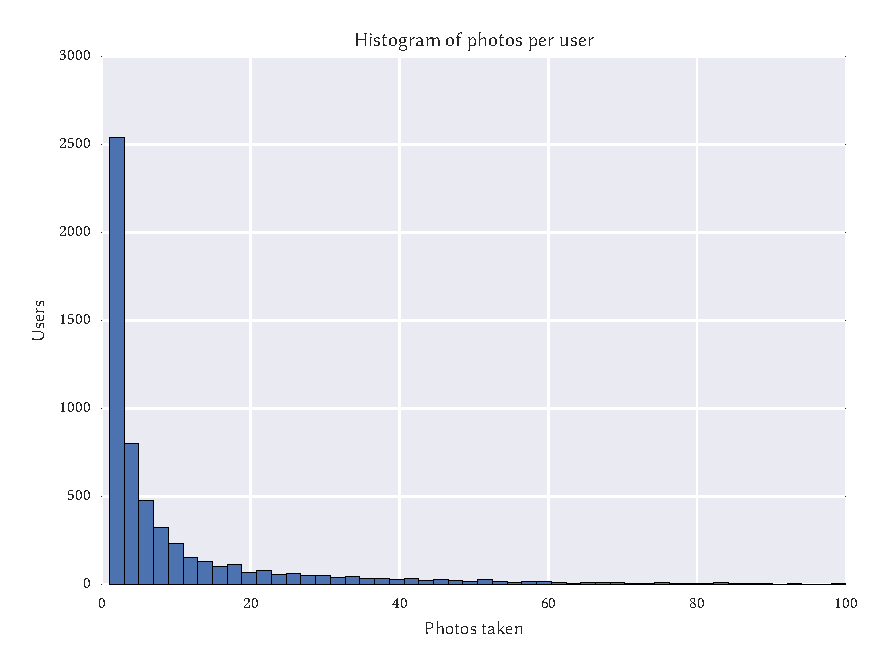
\includegraphics[width=\textwidth]{histogram_photos_per_user}
  \caption{Histogram of photos taken per user.}
  \label{fig:photo_user_distribution}
\end{figure}

\section{Path Finding}
\label{sec:path_discovery}

The photos collected in the previous section were used to identify the important locations that are often photographed by many people. These locations define the ground set $V$ for the models. In order to identify the popular locations automatically, the method proposed by \citet{Kleinberg2009} was used.

\citet{Kleinberg2009} define the problem of finding highly-photographed locationes as a clustering problem in a two-dimensional feature space, namely the space defined by the spatial coordinates of each photo. The clustering method used for this problem is mean-shift clustering, which was described in the background section.

Scikit\footnote{\url{http://scikit-learn.org/stable/}} was used for the mean-shift clustering implementation. The clustering was performed on the complete photo dataset with the unnormalized latitude and longitude features using a uniform disc as the kernel. The kernel bandwidth was 0.001 degrees which approximately represents a radius of 100m without significant errors for the geographic scale of Zürich.

The clustering procedure yielded 2686 clusters covering 137019 photos, the left over photos represent outliers that are not inside any of the resulting kernels. Figure \ref{fig:photos_per_clusters} displays a histogram of photos per cluster, it shows that over half of the clusters only contain one or two photos. This indicates that many of the clusters are actually not landmarks or highly photographed places, so in order to concentrate the model around the most interesting locations only the top $N$ clusters sorted by the number of photos were used.

\begin{figure}
  \centering
  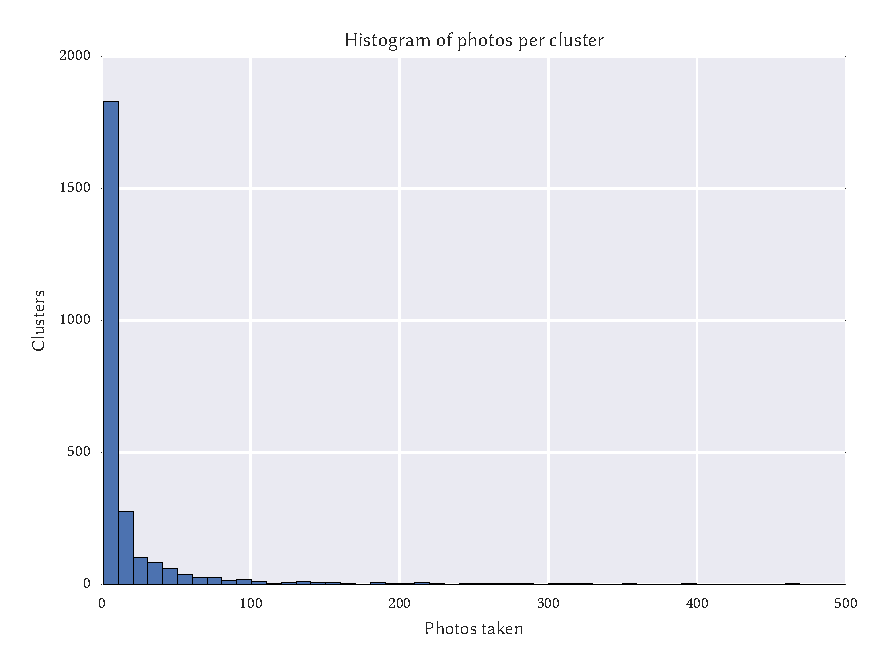
\includegraphics[width=\textwidth]{histogram_photos_per_cluster}
  \caption{Histogram of the number of photos per cluster. The graph is cut off at 500 because the distribution has a heavy tail.}
  \label{fig:photos_per_clusters}
\end{figure}

Two datasets were constructed, a small one with the top 10 clusters and a large one with the top 100 clusters. The small dataset was heavily used during the development of the models to test the implementation and try out different settings. On the other hand, the large dataset was mainly used for assessing the quality of the final models and comparing it against the baseline models.

Figures \ref{fig:top_10_zurich} and \ref{fig:top_100_zurich} show the selected clusters in the small and large setting, respectively. Additionally, Table \ref{tab:top_10_clusters} presents additional information about the top 10 clusters in the small dataset.

\begin{figure}
  \centering
  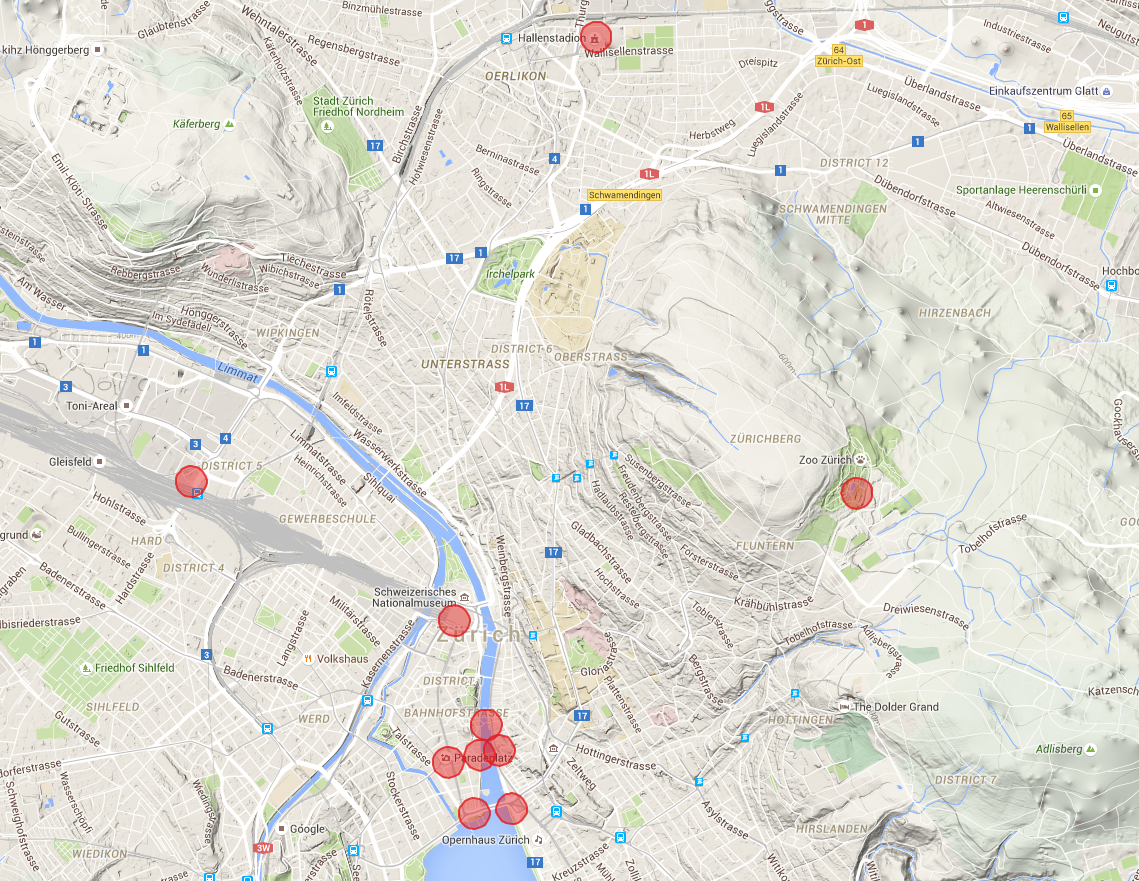
\includegraphics[width=\textwidth]{top_10_zurich}
  \caption{Top 10 clusters in Zürich according to the photo count.}
  \label{fig:top_10_zurich}
\end{figure}

\begin{figure}
  \centering
  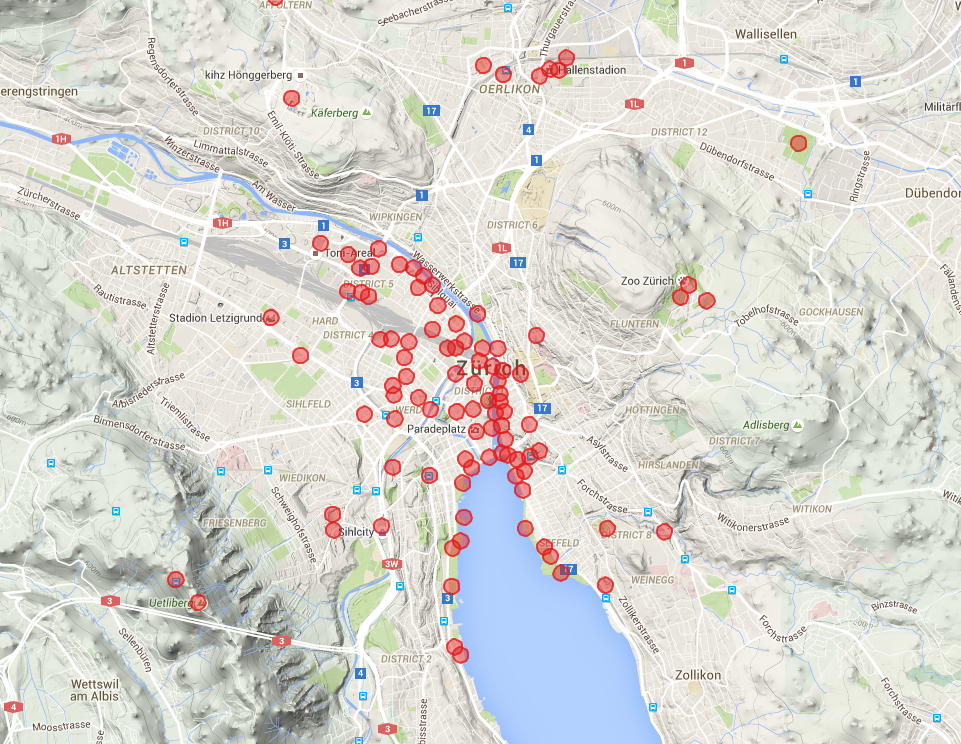
\includegraphics[width=\textwidth]{top_100_zurich}
  \caption{Top 100 clusters in Zürich according to the photo count.}
  \label{fig:top_100_zurich}
\end{figure}


\begin{table}
  \centering
  \caption{Top 10 clusters for Zürich.}
  \begin{tabular}{@{}lll@{}}
    \toprule
    Landmark & Photos taken & Unique users  \\
    \midrule
    Hauptbahnhof (Main train station) & 4224 & 932 \\
    Grossmünster (Church) & 3797 & 951 \\
    Bürkliplatz (Outdoors) & 3728 & 612 \\
    Hallenstadion (Event venue) & 3575 & 82 \\
    Fraumünster (Church) & 3414 & 889 \\
    Bellevueplatz (Outdoors) & 2584 & 437 \\
    Rathaus (Town hall) & 2569 & 690 \\
    Zoo & 2462 & 151 \\
    Paradeplatz (Outdoors) & 2372 & 438 \\
    Prime Tower & 1930 & 257 \\
    \bottomrule
  \end{tabular}
  \label{tab:top_10_clusters}
\end{table}

To extract the paths taken by individual users from the photo dataset, the procedure was as follows:

\begin{enumerate}
  \item The photos were grouped by user and date when they were taken.
  \item The photos in each user and date group represent a single path, ordered by date and time.
  \item The photos were replaced in the sequences by their corresponding clusters, including the cluster only once. If the photo did not belong to one of the top clusters, then the photo would be discarded.
  \item The resulting sequence of clusters represent the paths taken by users through the city.
\end{enumerate}

These sequences were used as the unordered sets for the set models, e.g. FLID, FLDC, or as ordered sequences for the Markov model baseline. Table \ref{tab:path-statistics} show the statistics for the final datasets.

\begin{table}
  \centering
  \caption{Path dataset statistics for Zürich.}
  \begin{tabular}{@{}lll@{}}
    \toprule
    & Small ($|V|=10$)& Large ($|V|=100$)  \\
    \midrule
    Included photos (\% of total) & 30655 (18\%) & 91661 (54\%)\\
    Paths extracted, i.e. $|\mathcal{D}|$ & 6781 & 16439 \\
    Singleton paths, i.e. $|S|=1$ & 5396 & 12927 \\
    Pair paths, i.e. $|S|=2$ & 799 & 1980 \\
    \bottomrule
  \end{tabular}
  \label{tab:path-statistics}
\end{table}

Additionally, Figures \ref{fig:histogram_path_length_10} and \ref{fig:histogram_path_length_100} show the histograms of the length of the sets in the small and large datasets, respectively. This shows that most of the sets are either singletons or pairs, which matches the fact that many users just take a few photos as it was shown in Figure \ref{fig:photo_user_distribution}.

\begin{figure}
  \centering
  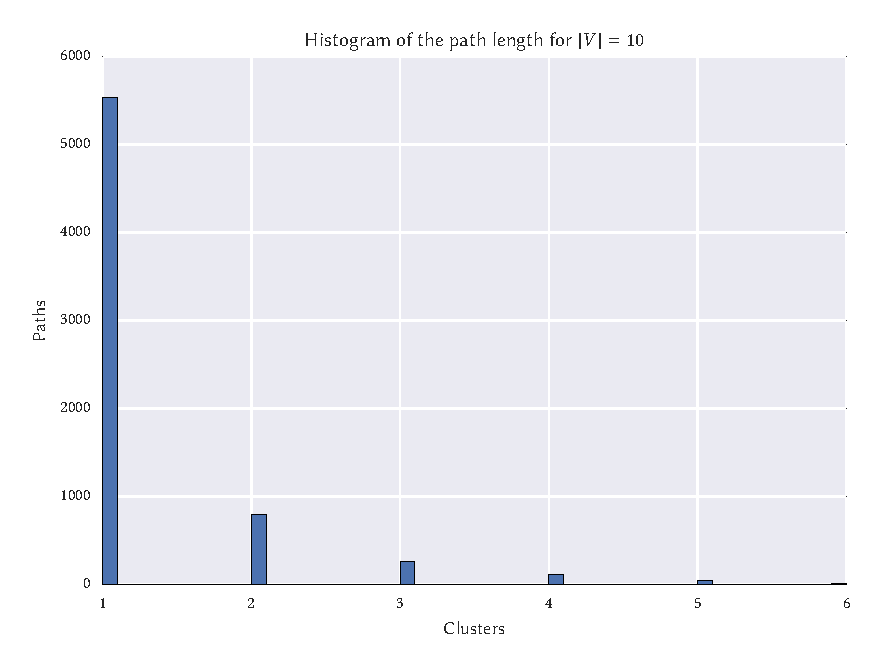
\includegraphics[width=\textwidth]{histogram_path_length_10}
  \caption{Histogram of set/path length for the small dataset.}
  \label{fig:histogram_path_length_10}
\end{figure}

\begin{figure}
  \centering
  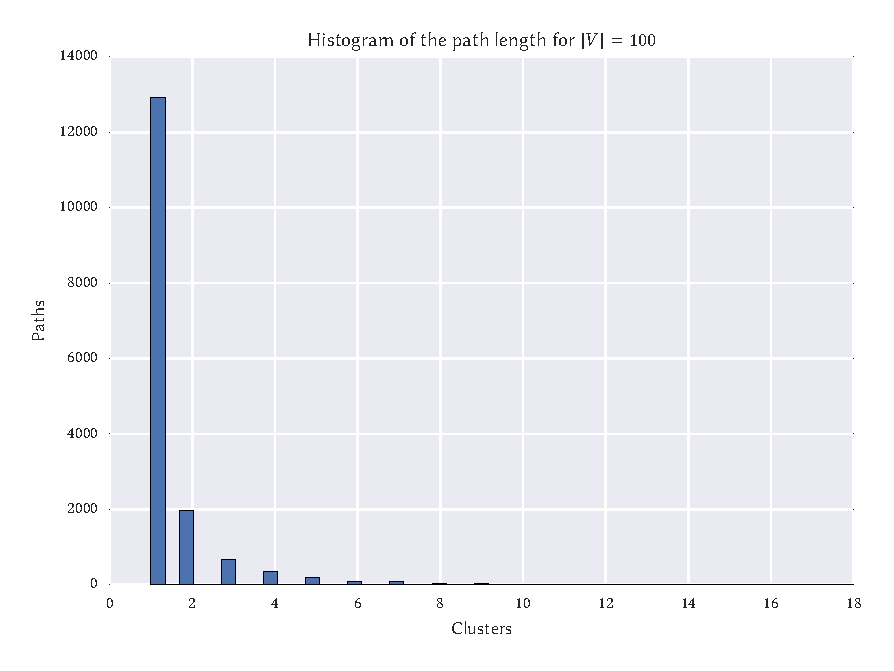
\includegraphics[width=\textwidth]{histogram_path_length_100}
  \caption{Histogram of set/path length for the large dataset.}
  \label{fig:histogram_path_length_100}
\end{figure}

\section{Models}

For the experiments, the FLID, FLDC and FFLDC models were used. The settings for these experiments will be presented in the next chapter along with the results. However, for all experiments the following implementation details were fixed:

\begin{itemize}
  \item The data was split in 8 random folds, with 90\% of the data used for training and 10\% for testing in each.
  \item The noise was generated using the log-modular model as described for the synthetic experiments.
\end{itemize}

\section{Baselines}
\label{sec:baselines}

This section describes the baseline models that were used as a comparison for the proposed models.

\subsection{Markov Chain}

A Markov chain can be used to model the behavior of Flickr users, assuming that each user selects the next location to visit and photograph only based on the current location, i.e. the Markov property. This model depends on the transition probabilities between the different landmarks in the dataset, concretely $P(l_{t+1} = i \mid l_{t} = j)$ where $l_{t+1}$ represents the next location and $l_{t}$ the current one. These probabilities can be estimated by counting all the occurrence of the transitions in the dataset, i.e.

\begin{equation}
  \hat{P}(l_{t+1} = i \mid l_{t} = j) = \frac{N(i,j)}{N(j)}
\end{equation}

Where $N(i,j)$ is the number of times that the location $i$ was photographed immediately after location $j$, and $N(j)$ is the number of times that location $N(j)$ was photographed. This model was used successfully by \citet{Kurashima2010} with good results for recommending tourists routes for a city based on Flickr data, therefore it is a natural choice for comparison against the newly proposed models. A full path can be constructed by selecting a starting location and choosing the next one according to the highest transition probability, then repeating the procedure until a desired length is reached.

Note that this model can be estimated efficiently from data, its running time is $\mathcal{O}(|\mathcal{D}|)$.

\subsection{Proximity Model}

Another, possibly naive, model is to assume that users photograph the next closest location to their current one. This can be useful to model paths that are concentrated in certain areas, for example in the Zürich dataset many of the paths only visit locations in the center and users seldom take photographs at the Zoo and a landmark in the center on the same day.

Formally, this model defines a series of transition probabilities $P(l_{t+1} = i \mid l_{1 \dots t})$ which are inversely proportional to the distance of the last visited location, i.e.

\begin{equation}
  P(l_{t+1} = i \mid l_{1 \dots t}) \propto \frac{1}{d(i, l_{t})}
\end{equation}

Where $d(i, j)$ is the distance between locations $i$ and $j$. Contrary to the Markov chain model, the proximity model takes into account the complete history of locations, this information is used to avoid going back to a previously visited location. The complete model is then defined by:

\begin{equation}
  \label{eq:proximity}
  P(l_{t+1} = i \mid l_{1 \dots t}) \propto \begin{cases}
    0 & \text{if}\ i \in l_{1 \dots t} \\
    \frac{1}{d(i, l_{t})} & \text{otherwise}
  \end{cases}
\end{equation}

This is a natural choice for a baseline model because it provides a very quick model that is not completely random, the probabilities in this model can be computed in $\mathcal{O}(|V|^{2})$ time, which is less than $|\mathcal{D}|$ for both datasets. To construct a path, the same procedure as for the Markov chain can be used.

\subsection{Log-modular Distribution}

As described before, a log-modular model is the simplest log-submodular model which makes it a natural comparison for the FLID and FLDC models. The log-modular model can also be used with features by solving the linear system in Equation \eqref{eq:modular_features} to make it comparable to the FFLDC model.

The log-modular can be estimated from data following the procedure defined in Section \ref{sec:learning_modular}, which only requires $\mathcal{O}(|\mathcal{D}|)$ time.

This model is significantly different from the two previous baselines because it does not model the order of the elements, simply the membership. However, it is also possible to build a path by first constructing a set of fixed size $n$ and then ordering the elements in order to minimize the total travel distance. A set of size $n$ can be constructed by selecting the $n$ locations with highest utility, i.e. $\argmax_{i} u_{i}$.

\section{Evaluation}
\label{sec:evaluation}

The evaluation of the models aims to assess their quality for the task of recommending additional locations to visit based on an initial set of locations that the user wants to visit. This recommendation can be structured as a path either directly from the output of the model, e.g. for the Markov chain case, or as a post-processing step, i.e. for the set based models.

The evaluation task is to predict the next location in a sequence given its first $n$ elements, this can be constructed by creating partial paths of increasing size from the paths in the test dataset and withholding the last element in the partial sequence. Thus each path of length $k$ generates $k-1$ partial paths for testing. For example the path $1,5,6$, generates 2 partial paths, namely $1$ and $1,5$, and the elements  to predict are $5$ and $6$, respectively. Note that only paths of at least size 2 are used in the task.

After each model is trained with the corresponding training dataset, the predictions for each partial path $S_{t} = [s_{1}, \dots, s_{t}]$ are made as follows:

\begin{description}
  \item[FLID, FLDC, FFLDC, Log-modular] The element with maximum probability, that is not already in the partial path is predicted, i.e. $\argmax_{i \notin S} P(S \cup \{i\})$ where $S$ is the set of the elements in the partial path $S_{t}$.
  \item[Markov Chain] The element with the highest transition probability with respect to the last element in the partial path is predicted, i.e. $\argmax_{i} P(i \mid s_{t})$.
  \item[Proximity] The element with the highest transition probability, i.e. minimum distance, with respect to the last element in the partial path is predicted, ignoring elements already in the sequence as defined in Equation \eqref{eq:proximity}.
\end{description}

The metric used for the quality of the predictions is overall accuraccy, i.e. the percentage of correct predictions. Formally, 

\begin{equation}
  Acc_{model} = \frac{1}{|\mathcal{T}|}\sum_{S_{t} \in \mathcal{T}}(\mathbb{I}_{\hat{s}_{t+1}, s_{t+1}})
\end{equation}

Where $\mathcal{T}$ is the set of all partial paths available for testing and $\mathbb{I}_{\hat{s}_{t+1}}$ is an indicator function that evaluates to 1 when the predicted element $\hat{s}_{t+1}$ is equal to the next element in the sequence $s_{t+1}$ and 0 otherwise.

Accuracy is the most used metric for recommender systems \citep{Herlocker2004} and it was the metric used by \citet{Kurashima2010} for evaluating single step recommendations in tourist routes. This accuracy metric also is similar to the leave-one-out procedured used by \citet{tschiatschek16learning} to evaluate the FLID model for product recommendation. Therefore, it is expected to provide a good assesment on the quality of the proposed models.
